% --
% game design

\section{Game Design}\label{sec:game_design}
\thesisStateNotReady
In this section the game design for the deployed KWS video game is presented.
Prior to explaining the game and its rules, it is important to mention the game menu and its vital settings for the input microphone device.
The game rules are explaining the win and loose condition of the video game.
Game mechanics restrict how the player can interact in the world and how to create actions for changing the states of game objects.
A level design describes and presents the actual levels of the game.


% --
% menu

\subsection{Menu}\label{sec:game_design_menu}
The main menu is the first screen that appears, when starting a video game. 
It usually consists of several selectable buttons that are referencing for instance to the start of the actual game, a link to the help menu or the options menu for graphic and music settings of the game.
The main menu and the help menu are shown in \rfig{game_design_menu_mainhelp}
\begin{figure}[!ht]
  \centering
  \subfigure[Main Menu]{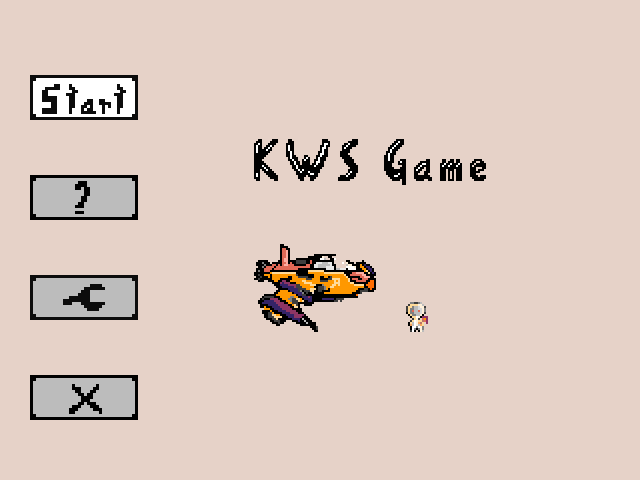
\includegraphics[width=0.40\textwidth]{./6_game/figs/game_design_menu_main}}
  \qquad
  \subfigure[Help Menu]{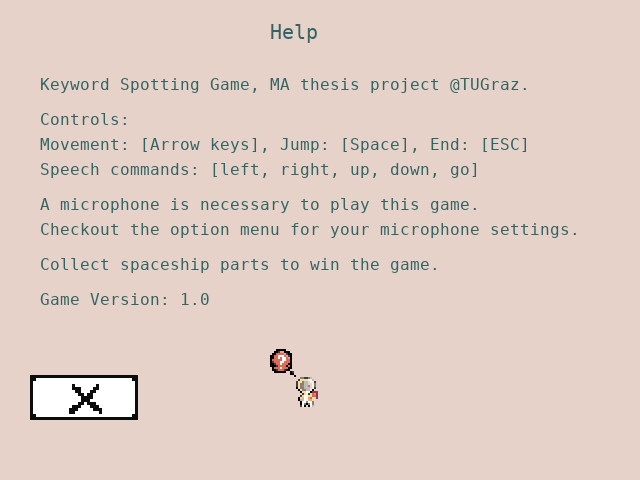
\includegraphics[width=0.40\textwidth]{./6_game/figs/game_design_menu_help}}
  \caption{Main and help menu of the KWS Game.}
  \label{fig:game_design_menu_mainhelp}
\end{figure}
\FloatBarrier
\noindent
With speech input deployed in a video game, the setting of the recording input device is useful to be added.
All available microphone input devices should be visualized in a list and being selectable for being able to switch between the independent devices.
Further a small visualization bar of the input signal energy from the selected device is beneficial, so that the user can verify its correct functionality.
An option for adjusting the energy threshold, by which the device detects the onset of a speech signal, must be added if this property is used within the video game.
The threshold must be adjustable because of varying recording amplification factors in different microphone set ups.
Another useful option screen for evaluating the output of the model by writing its corresponding output action onto the display is very beneficial for the player to test and understand its KWS ability.
All option menu screens are shown in \rfig{game_design_menu_options}
\begin{figure}[!ht]
  \centering
  \subfigure[Speech Commands]{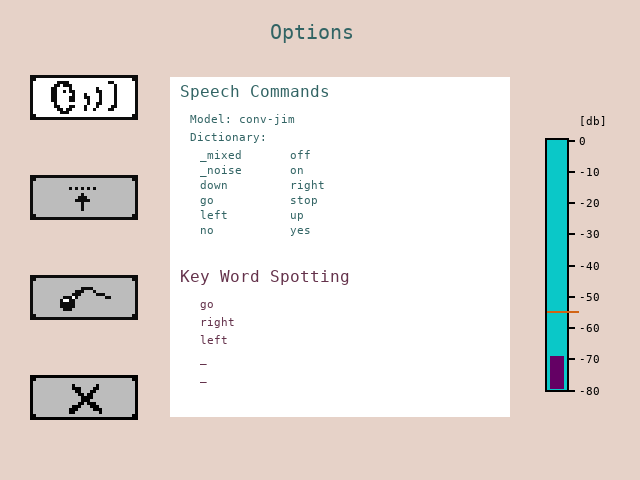
\includegraphics[width=0.40\textwidth]{./6_game/figs/game_design_menu_options_command}}
  \qquad
  \subfigure[Threshold]{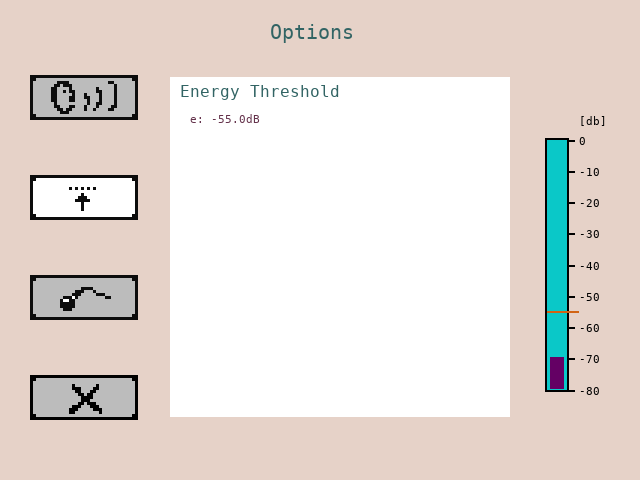
\includegraphics[width=0.40\textwidth]{./6_game/figs/game_design_menu_options_thresh}}
  \qquad
  \subfigure[Device]{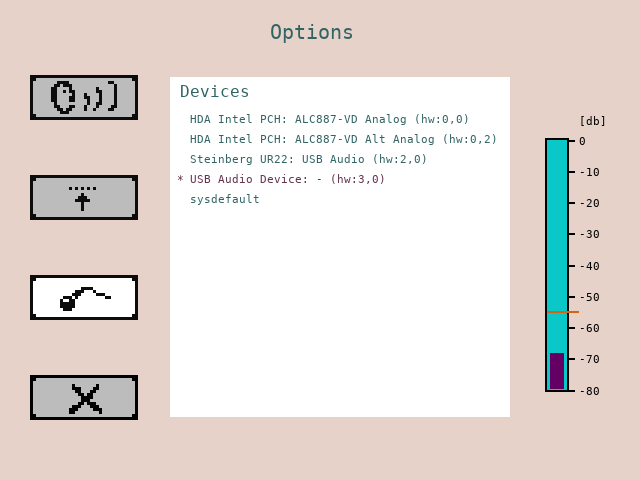
\includegraphics[width=0.40\textwidth]{./6_game/figs/game_design_menu_options_device}}
  \caption{Option menu with screens for the input device, the energy threshold and a KWS screen for analyzing the speech input classification.}
  \label{fig:game_design_menu_options}
\end{figure}
\FloatBarrier
\noindent


% --
% game rules

\subsection{Game Rules}\label{sec:game_design_rules}
The game rules were hold simple, so that the game part does not take too much effort to implement.
A simple adventure game in a 2D-platformer view (movement are left-right and jump, like the classical \enquote{Super Mario} games) was implemented, where the player has to collect objects and dodge enemies.
The win condition is to complete each individual level by collecting a single object within. 
The loose condition on the other hand is to collide with the enemy a single time.
If the player runs into the enemy, a loose screen appears and the same level can be restarted from its initial state.
Being able to reach the collectable objects, the player has to use speech commands.
Further descriptions are presented below in the game mechanics and the level design.


% --
% game mechanics

\subsection{Game Mechanics}\label{sec:game_design_mechanics}
The game mechanics with KWS are a highly time restricted, because of the processing time of the speech signals.
In this thesis the KWS system was used as augmented input control.
With standard keys for movement on the keyboard, the controlling of the character is handled, so that the player receives immediate feedback. 
For other more special actions, that do not require immediate feedback, a KWS control was applied.

The game mechanic implemented in the deployed video game, is to perform a two dimensional grid move upon a so called moveable block, by saying the command word (key word) of the intended direction, as for instance \enquote{left} and \enquote{right} or \enquote{up} and \enquote{down}.
A level can include several moveable blocks and the switch between those can be done by speaking the command word \enquote{go} until the desired moveable block is selected.
The selected movable block is highlighted with a different color as well as all moveable blocks share a common base color to distinguish them from ordinary walls.
At all times only one of all moveable block can be controlled by the player.

If a player does pronounce a word that does not corresponding to a movement, for instance \enquote{yes}, or a word that is not in the dictionary, hence corresponds to the \enquote{\_mixed} label, a small bubble with a question mark is shown for few frames next to the player character.
The indication of the \enquote{\_noise} label is done similarly, but with a bubble that includes a spiral intended as rubbish inputs symbol.
Both bubbles and the player is shown in \rfig{game_design_mechanic_bubble}.
\begin{figure}[!ht]
  \centering
  \subfigure[\enquote{\_mixed}]{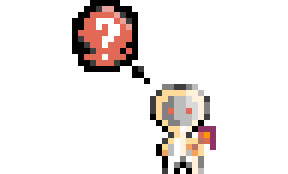
\includegraphics[height=0.15\textwidth]{./6_game/figs/game_design_mechanic_bubble_question}}
  \hspace{3cm}
  \subfigure[\enquote{\_noise}]{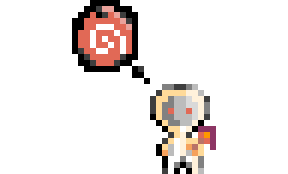
\includegraphics[height=0.15\textwidth]{./6_game/figs/game_design_mechanic_bubble_rubbish}}
  \caption{Handling of the \enquote{\_mixed} and \enquote{\_noise} label.}
  \label{fig:game_design_mechanic_bubble}
\end{figure}
\FloatBarrier
\noindent

Being able to provide a loose condition within the game, enemies were implemented.
If an enemy touches the player, the game is over and the actual level has to be restarted.
The player can perform a jump to dodge the enemy.
The movement of the enemy is to run from left to right and changing its direction when an obstacle is hit (like a wall).
The enemy sprite sheet is shown in \rfig{game_design_mechanic_enemy}.
\begin{figure}[!ht]
  \centering
  
\includegraphics[height=0.08\textwidth]{./6_game/figs/game_design_mechanic_enemy}
  \caption{Enemy sprite sheet.}
  \label{fig:game_design_mechanic_enemy}
\end{figure}
\FloatBarrier
\noindent


% --
% level design

\subsection{Level Design}\label{sec:game_design_level}
Two levels were implemented with the game mechanic of movable blocks, as described previously in \rsec{game_design_mechanics}.
The first level requires the player to learn how the game works and to move blocks out of the players path to the collectable object.
In the second level the player has to align the moveable blocks, such that by jumping upon them, higher plateaus can be reached.
The levels are both shown in \rfig{game_design_level}.
\begin{figure}[!ht]
  \centering
  \subfigure[Level One]{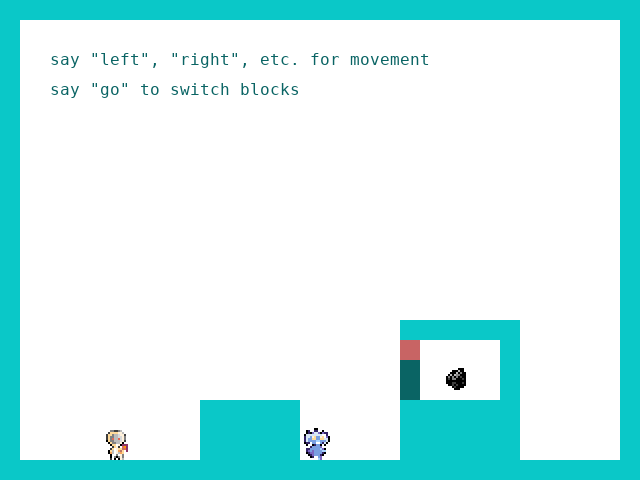
\includegraphics[width=0.40\textwidth]{./6_game/figs/game_design_level_one_start}}
  \qquad
  \subfigure[Level Two]{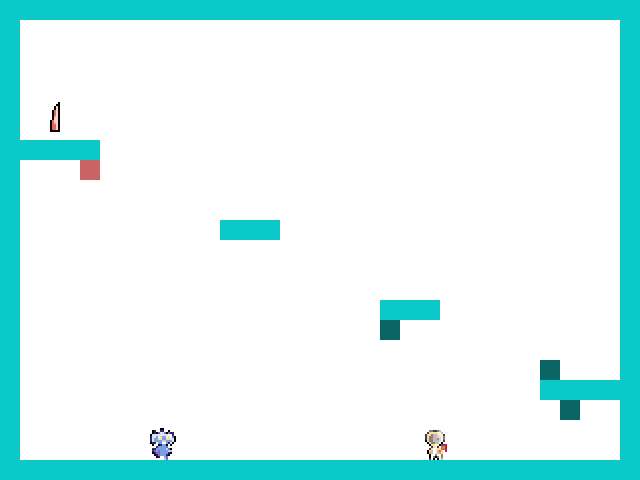
\includegraphics[width=0.40\textwidth]{./6_game/figs/game_design_level_two_start}}
  \caption{Level design of the implemented levels.}
  \label{fig:game_design_level}
\end{figure}
\FloatBarrier
\noindent
The completion of one level is done by collecting one specific object in the game.
A screen that shows the spaceship plus the collected part appears and the player has to press enter to go to the next level.
If the player collides with an enemy, a simple loosing screen appears and the player has to retry the same level.
Both scenarios with dedicated complete and loose screen of level one is shown in \rfig{game_design_level_complete}.
\begin{figure}[!ht]
  \centering
  \subfigure[Level One Complete]{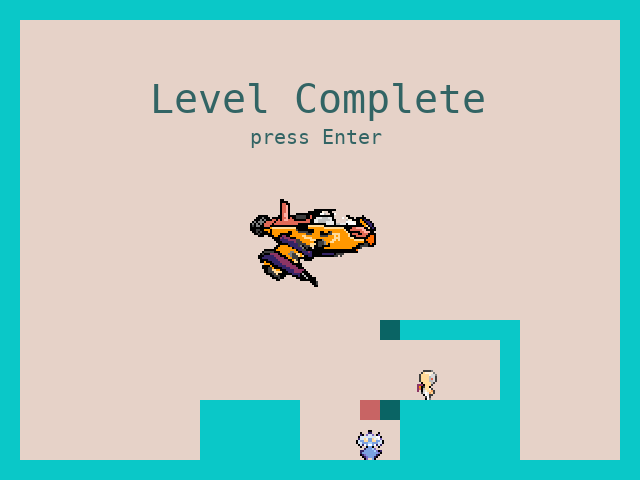
\includegraphics[width=0.40\textwidth]{./6_game/figs/game_design_level_one_complete}}
  \qquad
  \subfigure[Level One Loose]{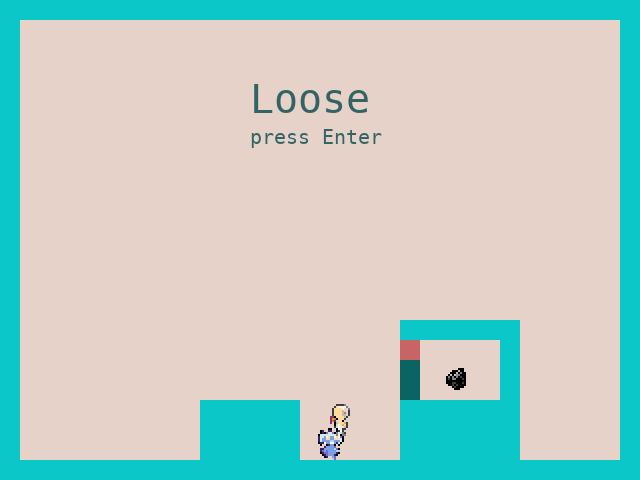
\includegraphics[width=0.40\textwidth]{./6_game/figs/game_design_level_one_loose}}
  \caption{Completing and loosing level one.}
  \label{fig:game_design_level_complete}
\end{figure}
\FloatBarrier
\noindent